\documentclass{ecnreport}

\stud{Control \& Robotics Master}
\topic{Manipulator Modeling \& Control}

\begin{document}

\inserttitle{Manipulator Modeling \& Control}
\insertsubtitle{Example for the RRRP robot}

\subsection*{Description of the robot}

The considered robot is the one seen during the lectures:
\begin{figure}[h!]\centering
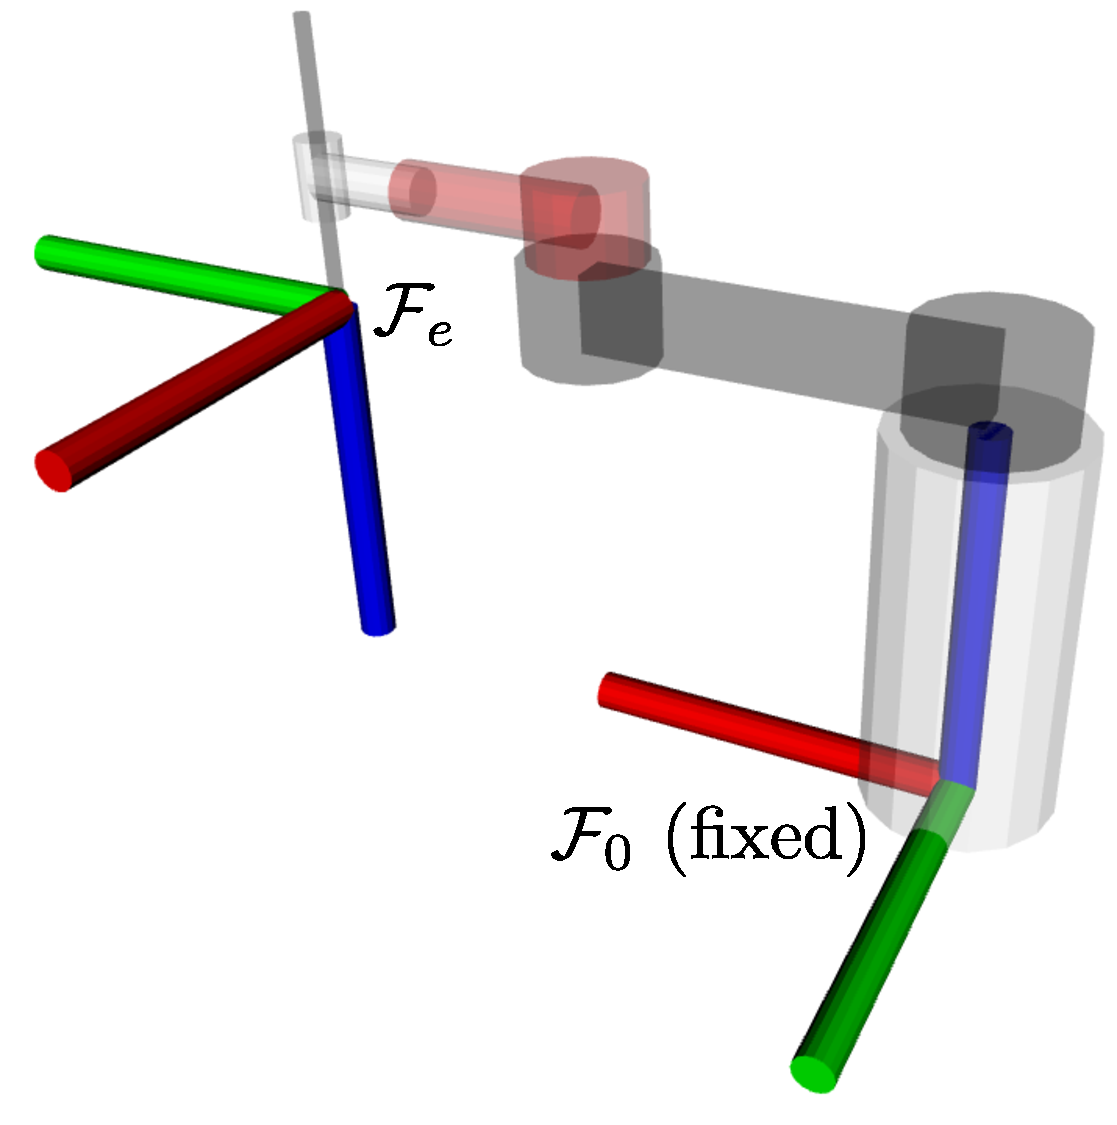
\includegraphics[height=.4\linewidth]{rrrp_rviz} \quad
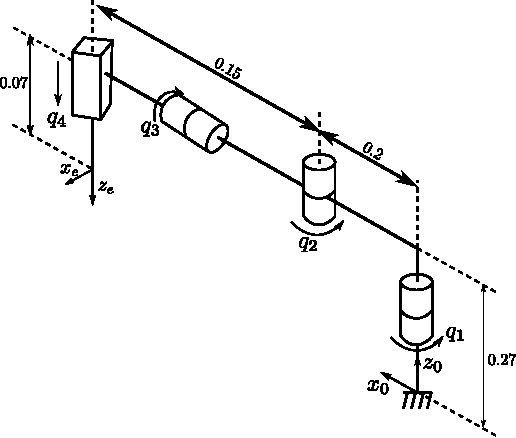
\includegraphics[height=.4\linewidth]{rrrp}   
\end{figure}

As we saw in class, the MDH table is as follows:
\begin{center}
\begin{tabular}{|c|c|c|c|c|}\hline
        Joint & $\alpha_i$ & $a_i$ &  $\theta_i$ & $r_i$\\\hline 
        1 & 0 & 0 & $q_1$ & $r_1$ \\\hline
        2 & 0& $a_2$  & $q_2+\pi/2$ & 0\\\hline
        3 & $\pi/2$ & 0 & $q_3$ & $r_3$\\\hline
        4 & $\pi/2$ & 0 & 0 & $q_4$\\\hline
        e & 0 & 0 & 0 & $r_4$\\\hline
    \end{tabular}
    with values: \begin{tabular}{|c|c|}\hline		
        $r_1$ & 0.27\\\hline
        $a_2$ & 0.2\\\hline
        $r_3$ & 0.15\\\hline
        $r_4$ & 0.07\\\hline
    \end{tabular}
\end{center}

The wrist-to-end effector transform is:
\begin{center}
$\Hom{w}{e} = \left[\begin{matrix}1 & 0 & 0 & 0\\
0 & 1 & 0 & 0\\0 & 0 & 1 & r_4\\0 & 0 & 0 & 1\end{matrix}\right]$
\end{center}

And the Direct Geometric model is:
\begin{center}
$\Hom{0}{4} = \Hom{f}{w} = \left[\begin{matrix}- s_{12} c_3 & c_{12} & - s_3 s_{12} & a_{2} c_1 - q_{4} s_3 s_{12} + r_{3} c_{12}\\c_3 c_{12} & s_{12} & s_3 c_{12} & a_{2} s_1 + q_{4} s_3 c_{12} + r_{3} s_{12}\\s_3 & 0 & - c_3 & - q_{4} c_3 + r_{1}\\0 & 0 & 0 & 1\end{matrix}\right]$
    \end{center}
    We of course have ${}^f\mathbf{M}_e = {}^f\mathbf{M}_w{}^w\mathbf{M}_e$

\subsection*{Solving the inverse model}

When solving the inverse model, we want to find $(q_1, q_2, q_3, q_4)$ that solve:\\
\begin{equation} \left[\begin{matrix}- s_{12} c_3 & c_{12} & - s_3 s_{12} & a_{2} c_1 - q_{4} s_3 s_{12} + r_{3} c_{12}\\c_3 c_{12} & s_{12} & s_3 c_{12} & a_{2} s_1 + q_{4} s_3 c_{12} + r_{3} s_{12}\\s_3 & 0 & - c_3 & - q_{4} c_3 + r_{1}\\0 & 0 & 0 & 1\end{matrix}\right] = \left[\begin{matrix}x_x & y_x & z_x & t_x\\x_y & y_y & z_y & t_y\\x_z & y_z & z_z & t_z\\0 & 0 & 0 & 1\end{matrix}\right]^* = {}^f\mathbf{M}_w^*
\label{model}
\end{equation}
Assuming that the right-hand side matrix is given with numerical values.

In order to do so, we have to identify remarquable equations types.

Terms of equation \eqref{model} can be obtained in C++ through:
\begin{cppcode}
 const auto [xx,xy,xz,yx,yy,yz,zx,zy,zz,tx,ty,tz] = explodeMatrix(fMe_des);
\end{cppcode}
where the \texttt{fMe\_des} is the numerical value of ${}^f\mathbf{M}_e^*$.

It will first apply ${}^f\mathbf{M}_w^* = {}^f\mathbf{M}_e^* \Hom{e}{w}$, then decompose it into all 12 values.



\subsubsection*{Solving for $\mathbf{q_3}$}

In \eqref{model} we notice: $\left\{\begin{array}{ll}s_3 &= x_z \\ -c_3 &= z_z\end{array}\right.$  \\
This can be written as a Type 3 equation:
\begin{equation*}
\left\{\begin{array}{l}X_1s_3+Y_1c_3 = Z_1 \\ X_2s_3+Y_2c_3 = Z_2\end{array}\right. \quad \text{ with } 
\left\{\begin{array}{ccc}
        X_1 = 1, & Y_1 = 0, & Z_1 = xz \\X_2 = 0, & Y_2 = -1, & Z_2 = zz
        \end{array}\right.
        \label{eq:q3}
\end{equation*} 
We can thus solve it for $q_3$ with the following syntax:
\begin{center}
    \cppstyle \raggedright
    \begin{lstlisting}
    for(auto q3: solveType3(1, 0, xz, 0, -1, zz))
    {
        // q3 is a valid solution, can be used to find other joints        
    
    }
    \end{lstlisting}
\end{center}

    \subsubsection*{Solving for $\mathbf{q_1}$ and $\mathbf{q_4}$}
    
    From a valid value for $q_3$, it is tempting to use $t_z$ to solve $q_4$. Indeed it would write:
    \begin{equation*}
    q_4 = \frac{r_1 - t_z}{\cos(q_3)}
    \end{equation*}Unfortunately this only works if $\cos(q_3) \neq 0$.\\
    On the opposite, we notice that $(t_x, t_y)$ form a system of two unkowns $(q_1, q_4)$:
    \begin{equation}
    \left\{\begin{array}{ll}
            a_{2} c_1 - q_{4} s_3 s_{12} + r_{3} c_{12} &= t_x \\  a_{2} s_1 + q_{4} s_3 c_{12} + r_{3} s_{12} &= t_y
            \end{array}\right.\label{eq:q14}
    \end{equation}While we do not know the values of $q_1$ and $q_2$, we know from \eqref{model} the values of $s_{12}$ and $c_{12}$.\\
    This makes \eqref{eq:q14} a Type 5 equation:
    \begin{equation*}
    \left\{\begin{array}{l}X_1s_1 = Y_1+Z_1q_4 \\ X_2c_1 = Y_2+Z_2q_4\end{array}\right. \quad \text{ with } 
    \left\{\begin{array}{ccc}
        X_1 = a_2, & Y_1 = t_y-r_3s_{12}, & Z_1 =-c_{12}s_3 \\X_2 = a_2, & Y_2 = t_x-r_3c_{12}, & Z_2 = s_{12}s_3
        \end{array}\right.
    \end{equation*}
    
    This is solved in practice with:
    \begin{center}
    \cppstyle \raggedright
    \begin{lstlisting}
    const auto s3 = sin(q3);    // we are inside the q3 loop so we know sin(q3)
    
    for(auto q14: solveType5(a2, ty-r3*yy, -yx*s3, a2, tx-r3*yx, yy*s3))
    {
        auto q1 = q14.qi;   // extract joint i = 1
        auto q4 = q14.qj;   // extract joint j = 4
    
    }
    \end{lstlisting}
\end{center}


\subsubsection*{Solving for $\mathbf{q_2}$ and adding the candidate solution}

The system $(y_x, y_y)$ will give the solutions of $q_1+q_2$ from a Type 3 equation. Then $q_2$ can easily be computed as we now have $q_1$. As we have a full candidate, we can add it to the potential solutions.

    \begin{center}
    \cppstyle \raggedright
    \begin{lstlisting}
    for(auto q12: solveType3(0, 1, yx, 1, 0, yy)
    {
        auto q2 = q12 - q1;
        addCandidate({q1, q2, q3, q4});
    }
    \end{lstlisting}
\end{center}


\end{document}
